\documentclass{article}
\usepackage[utf8]{inputenc}
\usepackage[top=2cm, bottom=2cm, outer=2cm, inner=2cm]{geometry}
\usepackage{graphicx}
\usepackage{url}
\usepackage{cite}
\usepackage{hyperref}
\usepackage{array}
\newcolumntype{x}[1]{>{\centering\arraybackslash\hspace{0pt}}p{#1}}

\usepackage{fancyhdr}
\pagestyle{fancy}
\fancyhf{}
\rhead{Bioinfomática}
\lhead{MSc. Vicente Machaca Arceda}
%\rfoot{Página \thepage}
\rfoot{\thepage}

% Logos in first page
\fancypagestyle{plain}{%
	\renewcommand{\headrulewidth}{0pt}%
	\fancyhf{}%
	\fancyfoot[C]{\footnotesize Page \thepage\ of \pageref{LastPage}}%
	\fancyhead[L]{ \raisebox{-0.2\height}{
\includegraphics[height=13mm]{../img/logo_unsa.jpg}}}
	\fancyhead[R]{ \raisebox{-0.2\height}{
\includegraphics[height=13mm]{../img/logo_epcc_unsa.png}}}
	\fancyhead[C]{  \fontsize{8}{8}\selectfont
		Universidad Nacional de San Agustín de Arequipa \\  
		\textbf{Escuela Profesional de Ciencia de la Computación} \\ 
		Curso: Computación Molecular Biológica 
		}
}


% para el codigo fuente
\usepackage{listings}
\usepackage{color}
\definecolor{dkgreen}{rgb}{0,0.6,0}
\definecolor{gray}{rgb}{0.5,0.5,0.5}
\definecolor{mauve}{rgb}{0.58,0,0.82}
\lstset{frame=tb,
  language=Python,
  aboveskip=3mm,
  belowskip=3mm,
  showstringspaces=false,
  columns=flexible,
  basicstyle={\small\ttfamily},
  numbers=none,
  numberstyle=\tiny\color{gray},
  keywordstyle=\color{blue},
  commentstyle=\color{dkgreen},
  stringstyle=\color{mauve},
  breaklines=true,
  breakatwhitespace=true,
  tabsize=3
}

\usepackage[english,french,spanish]{babel}
\AtBeginDocument{\selectlanguage{spanish}}
\renewcommand{\figurename}{Figura}
\renewcommand{\refname}{Referencias}
\renewcommand{\tablename}{Tabla}


% para la imagen de fondo
\usepackage{eso-pic}
\newcommand\BackgroundPic{%
\put(0,0){%
\parbox[b][\paperheight]{\paperwidth}{%
\vfill
\centering

\includegraphics[width=\paperwidth,height=\paperheight]{../img/background4.png}%
\vfill
}}}


\title{\textbf{Práctica 1}}
\author{MSc. Vicente Machaca Arceda}
\date{\today}

	

\begin{document}
	
% image background
%%%%%%%%%%%%%%%%%%%%%%%%%%%%%%%%%%%%%%%%%%%%%%%%%%%%%%%%%%%%%%%%%%%%%%%%%%	
%%%%%%%%%%%%%%%%%%%%%%%%%%%%%%%%%%%%%%%%%%%%%%%%%%%%%%%%%%%%%%%%%%%%%%%%%%	
%\AddToShipoutPicture{\BackgroundPic}
%\AddToShipoutPicture*{\BackgroundPic} %solo laprimera página
%%%%%%%%%%%%%%%%%%%%%%%%%%%%%%%%%%%%%%%%%%%%%%%%%%%%%%%%%%%%%%%%%%%%%%%%%%	
%%%%%%%%%%%%%%%%%%%%%%%%%%%%%%%%%%%%%%%%%%%%%%%%%%%%%%%%%%%%%%%%%%%%%%%%%%	



\maketitle

\begin{table}[h]
\begin{tabular}{|x{5cm}|x{6cm}|x{5cm}|}
\hline 
\textbf{DOCENTE} & \textbf{CARRERA}  & \textbf{CURSO}   \\
\hline 
MSc. Vicente Machaca Arceda & Escuela Profesional de Ciencias de la Computación & Computación Molecular Biológica    \\
\hline 
\end{tabular}
\end{table}

\begin{table}[h]
\begin{tabular}{|x{5cm}|x{6cm}|x{5cm}|}
\hline 
\textbf{PRÁCTICA} & \textbf{TEMA}  & \textbf{DURACIÓN}   \\
\hline 
01 & Dot Matrix & 3 horas   \\
\hline 
\end{tabular}
\end{table}


\section{Objetivos}
\begin{itemize}
    \item Comprender la importancia de los métodos de alineamiento de secuencias.
    \item Utilizar algunas herramientas de alineamiento de secuencias en linea.
    \item Implementar el método de \textit{Dot matrix}.
\end{itemize}


\section{Temas a tratar}
\begin{itemize}
    \item Alineamiento de secuencias.
    \item Algoritmo de \textit{Dot matrix}.
\end{itemize}

\section{Materiales}
\begin{itemize}
    \item Python
    \item Matplotlib 
    \item Numpy 
    \item BioPython
    \item Cuenta en Github
\end{itemize}

\section{Presentación del trabajo}
\begin{itemize}
    \item Se debe elaborar un informe en Latex donde se responda a cada ejercicio de la Sección \ref{sec:ejercicios}.
    \item En el informe se debe agregar un enlace al repositorio Github donde esta el código 
\end{itemize}

\clearpage

\section{Marco teórico}

\subsection{Alineamiento de secuencias}
Las secuencias de ADN y proteína definen la función de las proteínas en los seres vivos. Cuando más similares sean dos secuencias más similares tenderán a ser las funciones de las proteínas codificadas por ellas. Las secuencias de un mismo gen en un conjunto de especies serán más distintas cuanto más alejadas filogenéticamente estén las especies comparadas. De esta manera, es de vital importancia los métodos aplicados para alineamiento de secuencias \cite{comav2020}. 

\subsection{Alineamiento global y local}
Hay dos tipos de alineamientos principales: globales y locales. En el global se intenta que el alineamiento cubra las dos secuencias completamente introduciendo los gaps que sean necesarios. 
\begin{itemize}
    \item  En el local se alinean sólo las zonas más parecidas.
    \item  El gobal sirve para alinear secuencias que se empiecen y acaben en la misma región, por ejemplo genes homólogos de especies similares.
\end{itemize}

El alineamiento local suele ser la mejor opción a no ser que se esté seguro de que las los secuencias deben de parecerse a lo largo de toda sus extensión. En muchos casos las secuencias homólogas se parecen sólo en las regiones más conservadas.

\subsection{Alineamiento con Dot matrix}
El método Dot matrix, es un algoritmo gráfico de alineamiento de secuencias, este permite visualizar las areas comunes entre dos secuencias mediante puntos y lineas verticales como se pueder en la Figura  \ref{img:dot} \cite{xiong2006essential}.

\begin{figure}[h]
 \centering
    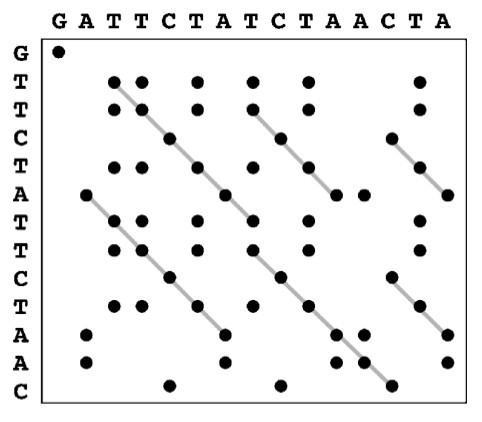
\includegraphics[width=\textwidth,height=0.2\textheight,keepaspectratio]{../img/alignment/dot.jpg}
    \caption{Dot matrix de dos secuencias de ADN. Los puntos representan las coincidencias de cada nucleotido y las lineas agrupan estas coincidencias.}
    \label{img:dot}
\end{figure}


\section{Actividades}

En esta ocasión vamos a descargar dos secuencias de proteinas y aplicaremos el algoritmo de Dot matrix.

\begin{enumerate}
    \item Busqueda de una secuencia de proteina Filamin-A de la especie \textit{Homo sapiens} desde la página: \href{https://www.uniprot.org/}{UniProt}  (Figura \ref{img:uniprot2})
    
    \begin{figure}[h]
     \centering
        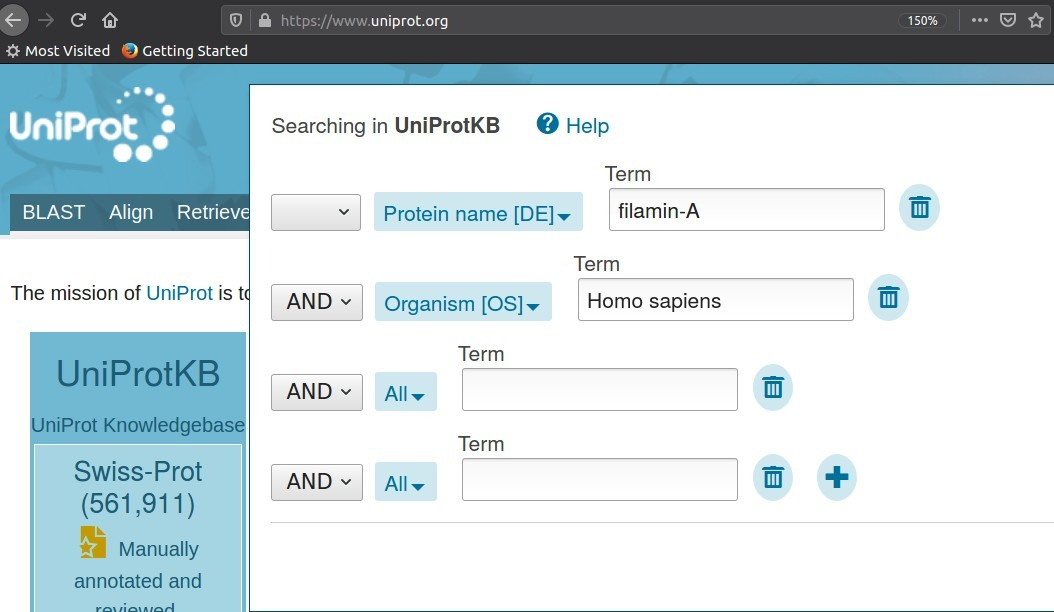
\includegraphics[width=\textwidth,height=0.3\textheight,keepaspectratio]{../img/alignment/uniprot2.jpg}
        \caption{Busqueda de la secuencia de la proteina Filamin-A de la especie Homo sapiens.}
         \label{img:uniprot2}
    \end{figure}
    
    \item Selecciona la secuencia  P21333 (si no existe, puede seleccionar otra secuencia).
    \item Busca el botón de descarga FASTA, de preferencia descarga el \textit{isoform} 1 (Figura \ref{img:uniprot4})
    
    \begin{figure}[h]
     \centering
        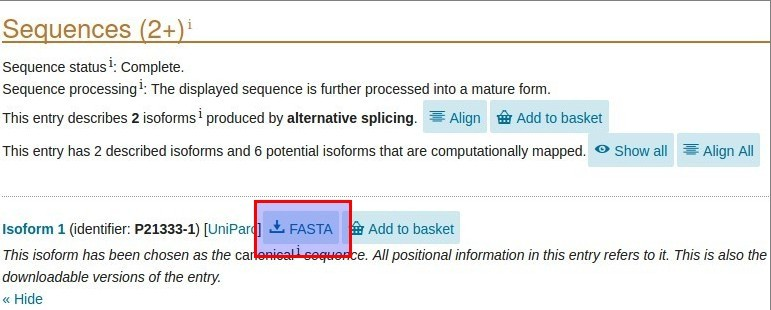
\includegraphics[width=\textwidth,height=0.2\textheight,keepaspectratio]{../img/alignment/uniprot4.jpg}
        \caption{Botón de descarga del archivo FASTA de la secuencia.}
        \label{img:uniprot4}
    \end{figure}
    
    \item Repetir los mismos pasos para la proteina Filamin-A de la especie \textit{mus musculus}, en este caso descargue de preferencia la secuencia: Q8BTM8 (Figura \ref{img:uniprot5})
    
    \begin{figure}[h]
     \centering
        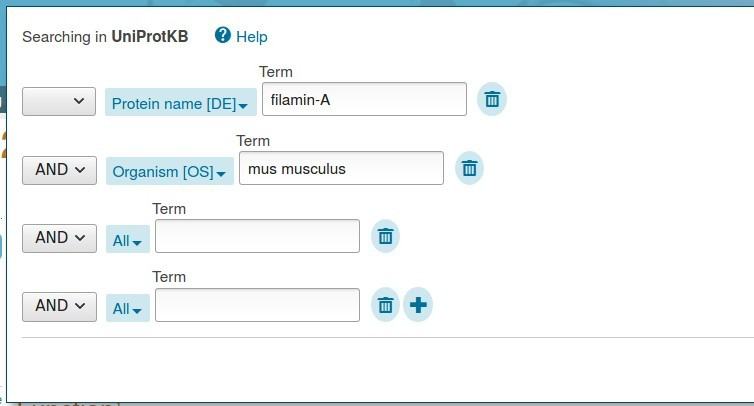
\includegraphics[width=\textwidth,height=0.3\textheight,keepaspectratio]{../img/alignment/uniprot5.jpg}
        \caption{Busqueda de la secuencia de la proteina Filamin-A de la especie mus musculus.}
        \label{img:uniprot5}
    \end{figure}
    
    \item Ingrese los archivos descargados en la página \href{http://bioinfo.nhri.org.tw/cgi-bin/emboss/dotmatcher}{DotMatcher} y genere el gráfico Dot matrix (Figura \ref{img:dot2})
    
    \begin{figure}[h]
     \centering
        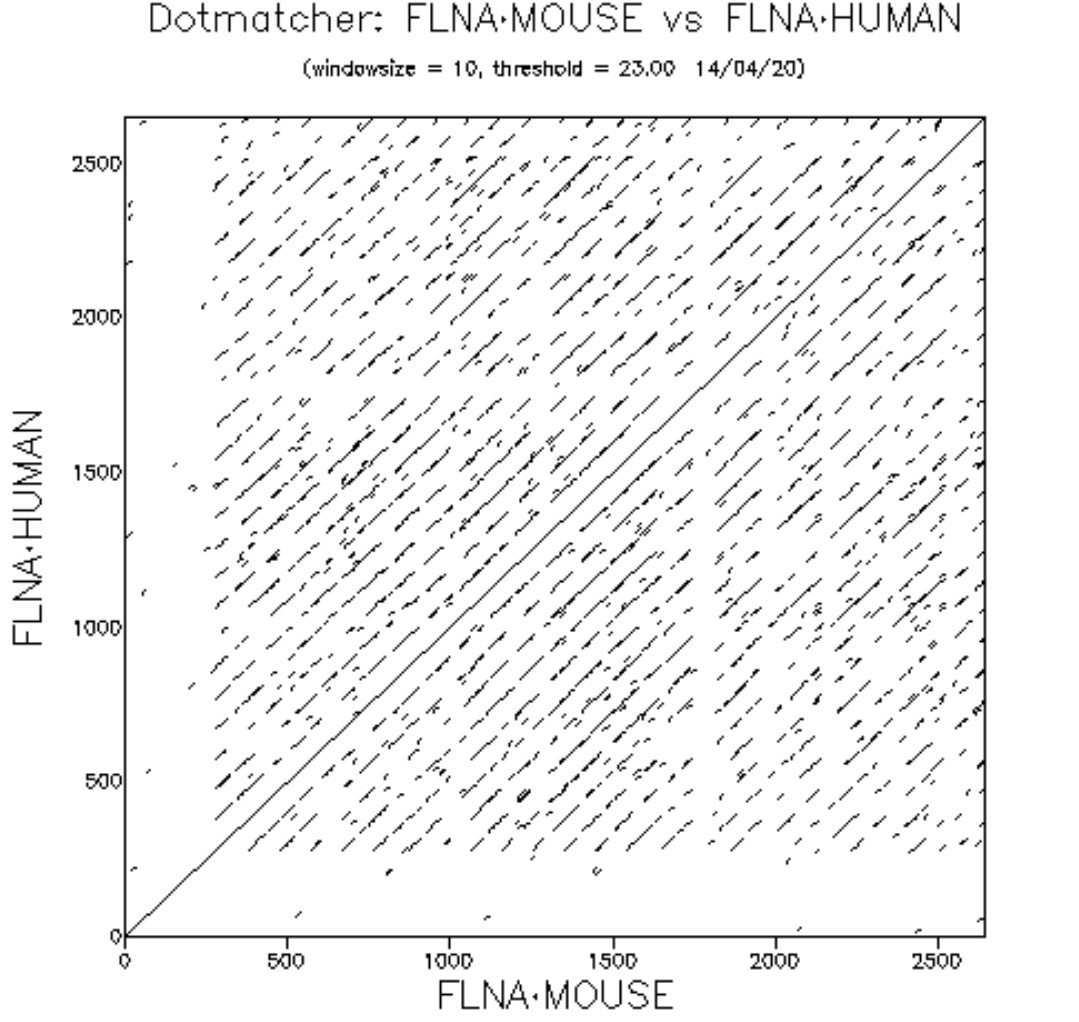
\includegraphics[width=\textwidth,height=0.4\textheight,keepaspectratio]{../img/alignment/dot2.jpg}
        \caption{Dot matrix de las secuencias Q8BTM8 y P21333.}
        \label{img:dot2}
    \end{figure}
   
\end{enumerate}


\section{Ejercicios}\label{sec:ejercicios}
\begin{enumerate}
 \item El siguiente código lee los 2 archivos descargados anteriormente y muestra las secuencias por pantalla.
    \begin{lstlisting}
    # dot_matrix.py
    from Bio import SeqIO

    sequences = SeqIO.parse("P21333.fasta", "fasta")
    for record in sequences:
        data1 = str(record.seq.upper()) # the fasta file just have one sequence 
    
    sequences = SeqIO.parse("Q8BTM8.fasta", "fasta")
    for record in sequences:
        data2 = str(record.seq.upper()) # the fasta file just have one sequence  
    
    print(data1)
    print(data2)
    \end{lstlisting}
 
    \item Ahora usted debe implementar un programa que genere un Dot matrix de manera similar a la Figura  \ref{img:dot2}. Se recomienda utilizar Matplot para la gráfica, de igual manera no es necesario dibujar las lineas, basta con dibujar los puntos por cada coincidencia.
    
    \item Descargue otras secuencias y genere el \textit{Dot matrix}, evalue sus resultados y comente.
\end{enumerate}


\clearpage
\bibliographystyle{ieeetr}
\bibliography{bibliography}

\end{document}
